%%%%%%%%%%%%%%%%%%%%%%%%%%%%%%%%%%%%%%%%%%%%%%%%%
%%%%%%%%%%%%%%%%%%% EXAMPLE 1 %%%%%%%%%%%%%%%%%%%
%%%%%%%%%%%%%%%%%%%%%%%%%%%%%%%%%%%%%%%%%%%%%%%%%

% Minimal example of a full HDR manuscript, in English
% Compile with: latexmk -lualatex -outdir=build main_hdr.tex
% See also "main_demand.tex" (short HDR demand, in French) and "main_phd.tex" (PhD manuscript)

%%%%%%%%%%%%%%%%%%%%%%%%%%%%%%%%%%%%%%%%%%%%%%%%%
%%%%%%%%%%%%%%%%% CONFIGURATION %%%%%%%%%%%%%%%%%
%%%%%%%%%%%%%%%%%%%%%%%%%%%%%%%%%%%%%%%%%%%%%%%%%

% Choose template
% Available document types: hdr, hdr_demand, phd -- available languages: english, french
\documentclass[hdr, english]{template/hdr}

% Extra colors
% These are only used in the example contents, feel free to remove them
\definecolor{phdColor}{HTML}{b8b806}%
\definecolor{postdocColor}{HTML}{e61b23}%
\definecolor{facultyColor}{HTML}{00b9df}%

%%%%%%%%%%%%%%%%%%%%%%%%%%%%%%%%%%%%%%%%%%%%%%%%%
%%%%%%%%%%%%%%%%%% INFORMATION %%%%%%%%%%%%%%%%%%
%%%%%%%%%%%%%%%%%%%%%%%%%%%%%%%%%%%%%%%%%%%%%%%%%

% Author
\setAuthorFirstName{Firstname}
\setAuthorName{Lastname}

% Affiliations
\setUniversity{Placeholder University}
\setDoctoralSchool{Placeholder Doctoral School}
\setDoctoralSchoolSubtitle{Information Sciences \& Technologies}
\addLogo{manuscript/covers/logo_university.png}{https://example.org}
\addLogo{manuscript/covers/logo_doctoral_school.png}{https://example.org}
\addLogo{manuscript/covers/logo_laboratory.png}{https://example.org}
\addLogo{manuscript/covers/logo_institute.png}{https://example.org}

% Document
\setDocumentTitle{A Placeholder Title for a Placeholder Manuscript}
\setDefenseDate{2026-11-12}

% Jury
% For an HDR, members are split between reviewers and examiners
\addReviewer{Firstname}{Reviewerone}{Senior Researcher, \acro{hdr}}{Placeholder Laboratory, Placeholder University}
\addReviewer{Firstname}{Reviewertwo}{Professor, \acro{hdr}}{Placeholder Institute}
\addReviewer{Firstname}{Reviewerthree}{Senior Researcher}{Placeholder Laboratory}
\addExaminer{Firstname}{Examinerone}{Researcher, \acro{hdr}}{Placeholder Institute}
\addExaminer{Firstname}{Examinertwo}{Professor, \acro{hdr}}{Placeholder University}

% Back cover elements
\setQRCodeLink{https://github.com/BastienPasdeloup/HDR-Template}
\setBackText{
    This text appears on the back cover, spread over two columns. Replace it with the abstract of your manuscript. Lorem ipsum dolor sit amet, consectetur adipiscing elit, sed do eiusmod tempor incididunt ut labore et dolore magna aliqua. Ut enim ad minim veniam, quis nostrud exercitation ullamco laboris nisi ut aliquip ex ea commodo consequat. Duis aute irure dolor in reprehenderit in voluptate velit esse cillum dolore eu fugiat nulla pariatur. Excepteur sint occaecat cupidatat non proident, sunt in culpa qui officia deserunt mollit anim id est laborum. Sed ut perspiciatis unde omnis iste natus error sit voluptatem accusantium doloremque laudantium, totam rem aperiam, eaque ipsa quae ab illo inventore veritatis et quasi architecto beatae vitae dicta sunt explicabo. Nemo enim ipsam voluptatem quia voluptas sit aspernatur aut odit aut fugit, sed quia consequuntur magni dolores eos qui ratione voluptatem sequi nesciunt.}

% Bibliography
% Each category groups the entries whose "usera" field matches the first argument
% Second argument is the letter used in the citation code, third one is the title of the section
\addBiblioCategory{thesis}{T}{\acro{phd} Theses}
\addBiblioCategory{book}{B}{Book Chapters}
\addBiblioCategory{journal}{J}{Journals}
\addBiblioCategory{conference}{C}{Conferences}
\addBiblioCategory{workshop}{W}{Workshops}
\addBiblioCategory{preprint}{P}{Preprints}

%%%%%%%%%%%%%%%%%%%%%%%%%%%%%%%%%%%%%%%%%%%%%%%%%
%%%%%%%%%%%%%%%%%%%% CONTENT %%%%%%%%%%%%%%%%%%%%
%%%%%%%%%%%%%%%%%%%%%%%%%%%%%%%%%%%%%%%%%%%%%%%%%

% Go
\begin{document}

    % Start with table of contents
    \tableofcontents

    % Chapters
    % Starred chapters are not numbered, and do not appear in the mini table of contents
% The optional argument in brackets is the label, used by \nameref
\chapter*[foreword]{Foreword}

\section*[tldr]{TL; DR}

This chapter is an unnumbered one, obtained with \verb|\chapter*[label]{Title}|.
Use it for a foreword, for the \nameref{acknowledgements} that follow, or for anything that should not carry a chapter number.
Such a chapter still takes a label, and is referred to exactly like a numbered one: \verb|\nameref{foreword}| gives \nameref{foreword}.

Lorem ipsum dolor sit amet, consectetur adipiscing elit, sed do eiusmod tempor incididunt ut labore et dolore magna aliqua.
Ut enim ad minim veniam, quis nostrud exercitation ullamco laboris nisi ut aliquip ex ea commodo consequat.

\section*[reading_guide]{How to Read This Document}

This document is meant to be read in its \acro{pdf} version, using a viewer able to display tooltips (\eg Acrobat, Evince, Overleaf).
Hovering an acronym or a citation then shows a short description, without having to jump to the end of the document.

\begin{itemize}
    \item \textbf{Acronyms} --- Every acronym is defined once in \verb|acronyms.tex|, and the ones this document uses are recalled in the list of \nameref{glossary}. In the text, \verb|\acro{ai}| gives \acro{ai}, \verb|\acrofull{ai}| gives \acrofull{ai}, and \verb|\acroname{ai}| gives \acroname{ai}.
    \item \textbf{References} --- Citations to my own work carry a code indicating the type of publication, \eg \cite{lastname2021journal} for a \textbf{J}ournal or \cite{lastname2022conference} for a \textbf{C}onference. External references appear like \cite{ipsum1998foundational}, and online resources like \cite{placeholder_www}.
    \item \textbf{Cross-references} --- Labels are declared as an optional argument of the sectioning command or environment, and recalled with \verb|\nameref|. For instance, \verb|\nameref{past}| gives \nameref{past}, and \verb|\nameref{example_figure}| gives \nameref{example_figure}. Unnumbered chapters are recalled by their title rather than by a number, which also applies to the two chapters closing the document: \verb|\nameref{bibliography}| gives \nameref{bibliography}, and \verb|\nameref{glossary}| gives \nameref{glossary}.
\end{itemize}

The template used for this document is available at \cite{template_repo}, under the \acro{gnu} \acro{gpl} v3.
Feel free to reuse it, and to replace all the placeholder text you find here.

    % Numbered chapter, with a label and an introductory text shown on the chapter page
\chapter[introduction]{Introduction}
 [
  The optional fourth argument of \textbackslash chapter is a short text displayed on the chapter page, above the mini table of contents. \\
  Use it to announce what the chapter contains, and to point to its sections, \eg \nameref{introduction_context} and \nameref{introduction_outline}.
 ]

\section[introduction_context]{Context}

Lorem ipsum dolor sit amet, consectetur adipiscing elit, sed do eiusmod tempor incididunt ut labore et dolore magna aliqua~\cite{ipsum1998foundational}.
Ut enim ad minim veniam, quis nostrud exercitation ullamco laboris nisi ut aliquip ex ea commodo consequat~\cite{tempor2009textbook}.

Duis aute irure dolor in reprehenderit in voluptate velit esse cillum dolore eu fugiat nulla pariatur.
Excepteur sint occaecat cupidatat non proident, sunt in culpa qui officia deserunt mollit anim id est laborum.

\begin{boxenv}[introduction_challenge]{Challenge}[Stating the problem in one sentence]
    Boxes are created with \texttt{\textbackslash begin\{boxenv\}[label]\{Type\}[Title]}.
    The type is free: a counter is created automatically for each distinct type, so this one is \nameref{introduction_challenge}.
    Boxes are also breakable, so a long one will span several pages without any special care.
\end{boxenv}

\section[introduction_contributions]{Contributions}

My contributions to this placeholder topic are summarized below, and detailed in \nameref{past}.

\begin{itemize}
    \item A placeholder method for placeholder data, published in \cite{lastname2021journal}.
    \item A placeholder analysis of placeholder models, published in \cite{lastname2022conference}.
    \item A placeholder application to a placeholder use case, published in \cite{lastname2019chapter}.
\end{itemize}

\section[introduction_outline]{Outline}

\nameref{past} summarizes my past activities, and \nameref{future} presents the directions I intend to follow.
Additional material is provided in \nameref{cv}.

    \chapter[past]{Overview of Past Activities}
 [
  This chapter is the showcase one: it demonstrates the figures, tables, equations, boxes and cross-references provided by the template. \\
  All the text is placeholder text, so do not look for any meaning in it. Replace it with a summary of your own activities.
 ]

\section[past_topic]{A First Research Topic}

\subsection[past_topic_context]{Context}

Lorem ipsum dolor sit amet, consectetur adipiscing elit~\cite{ipsum1998foundational}.
Sed do eiusmod tempor incididunt ut labore et dolore magna aliqua, as later formalized in \cite{tempor2009textbook} and revisited by \cite{amet2017seminal}.
My own contributions on this topic are \cite{lastname2015thesis}, \cite{lastname2021journal} and \cite{lastname2022conference}.

\begin{boxenv}[past_definition]{Definition}[Placeholder object]
    A \emph{placeholder object} is any object that carries no meaning, and only exists to occupy the space where a real one will eventually be written.
    Note that the counter of this box is independent from the one of \nameref{introduction_challenge}, since the types differ.
\end{boxenv}

Placeholder objects satisfy the property stated in \nameref{past_theorem}, whose proof is immediate.

\begin{boxenv}[past_theorem]{Theorem}[Conservation of placeholders]
    Let $\mathcal{P}$ be a set of placeholder objects, and $f$ a placeholder map.
    Then $f(\mathcal{P})$ is a set of placeholder objects.
\end{boxenv}

\begin{proof}{past_theorem}
    By definition, a placeholder object carries no meaning.
    Applying a placeholder map to a meaningless object cannot create meaning, hence the result.
\end{proof}

\subsection[past_topic_method]{Method}

The overall pipeline is sketched in \nameref{example_diagram}: a placeholder object, as introduced in \nameref{past_definition}, is fed to a placeholder model that produces a placeholder output.
The placeholder loss we minimize is given in \nameref{past_equation}, where $\bm{x}$ denotes an input, $\bm{y}$ its target, and $\theta$ the parameters of the model.

\begin{equation}[past_equation]
    \mathcal{L}(\theta) = \frac{1}{N} \sum_{i = 1}^{N} \left\| f_\theta(\bm{x}_i) - \bm{y}_i \right\|_2^2 + \lambda \left\| \theta \right\|_2^2
\end{equation}

Note that equations, figures and tables are numbered continuously across the whole document, and not per chapter.
This is on purpose: it makes cross-references such as \nameref{past_equation} unambiguous.

\paragraph[past_topic_runin]{Run-in headings} Below \texttt{\textbackslash subsubsection}, two run-in levels are available. This one is a \texttt{\textbackslash paragraph}: bold, in the colour of the titles, and referable like any other level through \nameref{past_topic_runin}.

\subparagraph{One level deeper} A \texttt{\textbackslash subparagraph} is the same run-in separator in the same colour, but in the normal font weight. Neither level is numbered, and neither appears in the table of contents.

\begin{figure}[example_diagram]{The pipeline used throughout this placeholder chapter. A figure is declared with \texttt{\textbackslash begin\{figure\}[label]\{caption\}}, and takes no placement specifier: the caption is the second, mandatory argument.}
    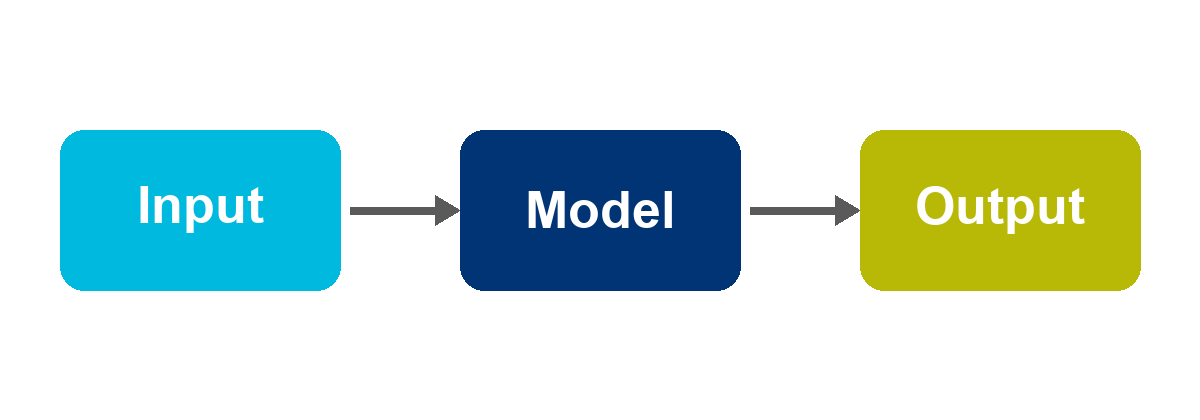
\includegraphics[width=0.9\linewidth]{manuscript/figures/example_diagram.png}
\end{figure}

\subsection[past_topic_results]{Results}

Results are reported in \nameref{example_figure}, and summarized in \nameref{example_table}.
As expected, the placeholder model in \nameref{example_figure}~\nameref{example_figure_curves} outperforms the placeholder baseline, which is exactly what a placeholder result is supposed to do.

\begin{figure}[example_figure]{A figure made of several subfigures. Subfigures take a label, a width, and a caption, and can be referred to individually, as in \nameref{example_figure_image}, or as a whole through \nameref{example_figure}.}
    \begin{subfigure}[example_figure_image]{0.48\linewidth}{A raster image, included with the usual \texttt{\textbackslash includegraphics}.}
        
\includegraphics[width=\linewidth]{manuscript/figures/example_image.png}
    \end{subfigure}
    \hfill
    \begin{subfigure}[example_figure_curves]{0.48\linewidth}{A vector figure, generated by a script and included with \texttt{\textbackslash input}. \nameref{example_plot_model} The placeholder model; \nameref{example_plot_baseline} The placeholder baseline. Both markers are placed with \texttt{\textbackslash labeledText[label]\{text\}}, and recalled here with \texttt{\textbackslash nameref}.}
        % Example of a vector figure, meant to be included with \input{} inside a figure environment
% Such fragments are typically produced by a script, so that data and rendering stay in sync
% The tikzpicture environment is patched by the template to never overflow \linewidth

\begin{tikzpicture}

    \begin{axis}
        [
            height      = 5cm,
            width       = \linewidth,
            xlabel      = {Number of training epochs},
            ylabel      = {Placeholder metric},
            xmin        = 0, xmax = 20,
            ymin        = 0, ymax = 1,
            grid        = major,
            grid style  = {separatorColor},
            legend pos  = south east,
            legend cell align = left,
        ]

        \addplot[titlesColor, line width=1.5pt, mark=*, mark size=1.5pt] coordinates
            {
                (0, 0.10) (2, 0.38) (4, 0.55) (6, 0.66) (8, 0.73)
                (10, 0.78) (12, 0.82) (14, 0.84) (16, 0.86) (18, 0.87) (20, 0.87)
            };
        \addlegendentry{Placeholder model}

        \addplot[linksColor, line width=1.5pt, dashed, mark=square*, mark size=1.5pt] coordinates
            {
                (0, 0.10) (2, 0.30) (4, 0.44) (6, 0.53) (8, 0.59)
                (10, 0.63) (12, 0.66) (14, 0.68) (16, 0.69) (18, 0.70) (20, 0.70)
            };
        \addlegendentry{Placeholder baseline}

    \end{axis}

\end{tikzpicture}

    \end{subfigure}
\end{figure}

\begin{table}[example_table]{Placeholder results, on placeholder datasets. Tables follow the same convention as figures: \texttt{\textbackslash begin\{table\}[label]\{caption\}}.}
    \begin{tabular}{lcc}
        \hline
        \textbf{Dataset} & \textbf{Baseline} & \textbf{Placeholder model} \\
        \hline
        Placeholder-A    & $0.70 \pm 0.02$   & $\bm{0.87 \pm 0.01}$       \\
        Placeholder-B    & $0.61 \pm 0.03$   & $\bm{0.79 \pm 0.02}$       \\
        Placeholder-C    & $0.55 \pm 0.04$   & $\bm{0.68 \pm 0.03}$       \\
        \hline
    \end{tabular}
\end{table}

\section[past_collaborations]{Collaborations}

Beyond \nameref{past_topic}, I contributed to a few placeholder collaborations, listed below.
\acro{cnn_plural} were involved in most of them, which is a convenient excuse to demonstrate a variation: \verb|cnn_plural| carries no \verb|long| field and names \verb|cnn| in its \verb|alt| field, so the list of \nameref{glossary} holds no line of its own for it. Hovering it still shows \acroname{cnn_plural}, and clicking it leads to the \acro{cnn} entry.

\begin{boxenv*}{\faFlask~\cite{lastname2019chapter}}[\fullcite{lastname2019chapter}]
    A starred box, \texttt{boxenv*}, is not numbered.
    This makes it convenient to summarize a publication: the title of the box is the citation, and its subtitle the full reference.
    Lorem ipsum dolor sit amet, consectetur adipiscing elit, sed do eiusmod tempor incididunt.
\end{boxenv*}

\begin{boxenv*}{\faFlask~\cite{lastname2023workshop}}[\fullcite{lastname2023workshop}]
    Ut enim ad minim veniam, quis nostrud exercitation ullamco laboris nisi ut aliquip ex ea commodo consequat.
    Duis aute irure dolor in reprehenderit in voluptate velit esse cillum dolore eu fugiat nulla pariatur.
\end{boxenv*}

Online resources can be cited the same way, \eg \cite{placeholder_www}, and are gathered in their own section of the \nameref{bibliography}.

    \chapter[future]{Future Work \& Directions}
 [
  A short chapter, to show that a chapter does not have to be long. \\
  It presents the directions I intend to follow after the work summarized in \nameref{past}.
 ]

\section[future_short_term]{Short Term}

Lorem ipsum dolor sit amet, consectetur adipiscing elit, sed do eiusmod tempor incididunt ut labore et dolore magna aliqua.
This direction directly extends \cite{lastname2025preprint}, and relies on the placeholder loss of \nameref{past_equation}.

\begin{boxenv}[future_challenge]{Challenge}[Making placeholders scale]
    The main obstacle is the cost of placeholder training, which grows with the number of placeholder objects.
    Note that this box continues the counter started by \nameref{introduction_challenge}, since both share the same type.
\end{boxenv}

\section[future_long_term]{Long Term}

Ut enim ad minim veniam, quis nostrud exercitation ullamco laboris nisi ut aliquip ex ea commodo consequat.
In the long run, I would like to address \nameref{future_challenge} by combining the results of \nameref{past_topic_results} with the \acro{sota} approaches of \cite{amet2017seminal}.

\begin{itemize}
    \item A first placeholder direction, on placeholder data.
    \item A second placeholder direction, on placeholder models.
    \item A third placeholder direction, on placeholder applications.
\end{itemize}


    % Appendices
    \appendices
    % Chapters declared after \appendices are numbered as appendices
\chapter[cv]{Curriculum Vitæ}
[
    An appendix behaves exactly like a chapter, except that it is numbered as an appendix and appears under a dedicated entry in the table of contents. \\
    This one shows the two-column layout used throughout the template for tabular material.
]

    \section[cv_info]{General Information}

        \begin{tabularx}{\linewidth}{r|X}
            \textbf{Name} & Firstname \textsc{Lastname} \\
            \textbf{Born} & \date{1988-10-03} \\
            \textbf{Nationality} & Placeholder \\
            \textbf{Links} & \href{https://example.org}{\faGlobeAmericas}
                             \hspace{\valparskip}\href{https://example.org}{\faGraduationCap}
                             \hspace{\valparskip}\href{https://example.org}{\faGithub} \\
            \textbf{Email} & \href{mailto:firstname.lastname@example.org}{\texttt{firstname.lastname@example.org}}
        \end{tabularx}

        Note the \verb|\date| command: it takes an ISO date and formats it according to the language of the document.

    \section[cv_education]{Education \& Positions}

        \begin{tabularx}{\linewidth}{r|X}
            \textbf{2010 -- 2015} & \acro{phd} in Placeholder Science \newline
                                    Placeholder Laboratory, Placeholder University \newline
                                    Dissertation: \cite{lastname2015thesis} \\
            \textbf{2015 -- 2017} & Postdoctoral researcher \newline
                                    Placeholder Institute \\
            \textbf{Since 2017} & Associate professor \newline
                                  Placeholder Laboratory, Placeholder University
        \end{tabularx}

    \section[cv_supervision]{Supervision}

        % \arrowBox draws a timeline: a colored ribbon on the left of an entry, carrying a
        % vertical label, and a two-column table of details on the right
        % Usage: \arrowBox{color}{ribbon label}{heading}{rows of the table}
        % - color        one of the extra colors declared in "main_hdr.tex"
        % - ribbon label the period the entry belongs to; consecutive entries of the same
        %                period repeat \raisebox{0.4ex}{\dots} instead, so that the ribbon
        %                reads as one continuous timeline
        % - heading      shown above the table, and greyed out: links stay colored, so an
        %                icon without a link (here GitHub) shows as unavailable
        % - rows         the body of a "r|X" tabularx, so use & and \\ as usual

        \subsection[cv_supervision_phd]{\acro{phd} Students}

            \arrowBox{facultyColor}{As Associate Professor}
            {
                \paragraph[cv_student_fourth]{Fourth \textsc{Student}}
                {\hspace{\valparskip}\href{https://example.org}{\faGraduationCap}}
                {\hspace{\valparskip}\href{https://example.org}{\faLinkedin}}
                {\hspace{\valparskip}\faGithub}
            }{
                \textbf{Period} & 2021 -- 2024 (36 months) \\
                \textbf{Defended} & \date{2024-11-29} \\
                \textbf{Share} & 50\% \\
                \textbf{Funding} & Placeholder Foundation \\
                \textbf{Subject} & \inquotes{A Placeholder Title for a Placeholder Thesis} \\
                \textbf{Publications} & \cite{lastname2023workshop, lastname2025preprint}
            }
            \arrowBox{facultyColor}{\raisebox{0.4ex}{\dots}}
            {
                \paragraph[cv_student_fifth]{Fifth \textsc{Student}}
                {\hspace{\valparskip}\href{https://example.org}{\faGraduationCap}}
                {\hspace{\valparskip}\faLinkedin}
                {\hspace{\valparskip}\href{https://example.org}{\faGithub}}
            }{
                \textbf{Period} & Since 2024 (in progress) \\
                \textbf{Share} & 33\% \\
                \textbf{Funding} & Placeholder Region (\inquotes{Placeholder} grant) \\
                \textbf{Subject} & Yet another placeholder subject
            }

        \subsection[cv_supervision_interns]{Interns}

            % Changing the color and the label starts a new period on the timeline
            \arrowBox{facultyColor}{As Associate Professor}
            {
                \paragraph[cv_intern_second]{Second \textsc{Coauthor}}
                {\hspace{\valparskip}\faGraduationCap}
                {\hspace{\valparskip}\href{https://example.org}{\faLinkedin}}
                {\hspace{\valparskip}\faGithub}
            }{
                \textbf{Period} & 2022 (6 months) \\
                \textbf{Level} & \acro{msc} 2 \\
                \textbf{Share} & 100\% \\
                \textbf{Subject} & \inquotes{Another Placeholder Topic}
            }
            \arrowBox{postdocColor}{As Postdoctoral Researcher}
            {
                \paragraph[cv_intern_third]{Third \textsc{Contributor}}
                {\hspace{\valparskip}\href{https://example.org}{\faGraduationCap}}
                {\hspace{\valparskip}\faLinkedin}
                {\hspace{\valparskip}\faGithub}
            }{
                \textbf{Period} & 2016 (4 months) \\
                \textbf{Level} & \acro{msc} 1 \\
                \textbf{Share} & 50\% \\
                \textbf{Subject} & A placeholder internship topic
            }
            \arrowBox{phdColor}{As \acro{phd} Student}
            {
                \paragraph[cv_intern_first]{First \textsc{Placeholder}}
                {\hspace{\valparskip}\faGraduationCap}
                {\hspace{\valparskip}\faLinkedin}
                {\hspace{\valparskip}\faGithub}
            }{
                \textbf{Period} & 2014 (3 months) \\
                \textbf{Level} & \acro{bsc} 3 \\
                \textbf{Share} & 100\% \\
                \textbf{Subject} & The very first placeholder internship
            }

    \section[cv_teaching]{Teaching}

        \begin{tabularx}{\linewidth}{r|X}
            \textbf{Since 2017} & \inquotes{Introduction to \acroname{ml}} \newline
                                  \acro{msc} 1, 30h/year \\
            \textbf{Since 2019} & \inquotes{Placeholder Programming} \newline
                                  \acro{msc} 2, 45h/year
        \end{tabularx}


    % Bibliography and glossary at the end
    \printbibliography
    \printglossaries

% Done
\end{document}
